% 请在下方的大括号相应位置填写正确的节标题和标签,以及作者姓名
\section{安装Python}\label{sec:安装Python}
\sectionAuthor{Jiaqi Z.}

% 请在下方的item内填写本节知识点
\begin{Abstract}
    \item 什么是Python程序语言
    \item 如何安装Python IDLE
    \item 如何安装Anaconda
\end{Abstract}

在本章,我们将讨论Python程序语言的基本语法(所谓基本语法,指的是Python程序语言本身所提供的编程语法,不包括后面所使用的库函数)。这一部分对于整个Python语言是基础,因此有必要仔细学习并掌握它们。

但在开始之前,让我们先来介绍一下Python语言。

Python由荷兰国家数学与计算机科学研究中心的Guido van Rossum(吉多·范罗苏姆)于1990年代初设计,作为一门叫做ABC语言的替代品。 

\begin{extend}
    ABC语言是Guido参加设计的一种教学语言,可以说是专门针对非专业程序员设计的。但是,ABC语言并没有成功,究其原因,Guido本人认为是由于其非开放造成的。因此,他本人决心在Python语言中避免这一错误。

    可以说,Python语言是从ABC语言发展而来,并结合了如Shell语言和C语言的习惯。
\end{extend}

Python语言目前已经称为最受欢迎的程序语言之一,在2019年1月,TIOBE编程语言排行榜将Python语言评为2018年度语言。由于Python语言的简洁性、易读性和可扩展性,在国外大多数科研机构都逐渐开始使用Python语言进行科学计算研究,同时,像麻省理工学院的计算机科学与编程导论课也使用Python语言讲授。同时,Python大量的科学计算扩展库也帮助科研人员使用(其中最著名的就是NumPy、Pandas和Matplotlib,分别用来进行数组矩阵处理,数值运算和绘图,在后面的章节我们也会介绍着三个库)。

Python语言具有如下特点:

\begin{itemize}
    \item 简单易学:Python语言极其容易上手,且接近自然语言;
    \item 免费、开源:Python语言是自由软件之一,你可以很容易下载到对应的源代码,并对其进行修改,并用于新的软件中;
    \item 高级语言:相较于C语言,Python语言没有指针等类似的概念,你不需要管理内存分配等底层细节;
    \item 可移植性:目前,Python语言已经被移植到如Linux、Windows、Mac OS操作系统中。在运行时,你不需要编译成二进制代码,而是直接从源代码中运行\footnote{从底层来看,Python实际上是将程序翻译成字节码(byte code),再使用如Python Virtual Machine(Python虚拟机)来执行这些字节码。这类似于Java语言的运行方式,但Python的虚拟机相较于操作系统本身更远,抽象程度更高。};
    \item 可扩展性:Python语言可以支持部分程序使用C/C++语言编写,然后提供对应的接口,从而在Python中调用C/C++语言;反之也可以(将Python语言用于C/C++语言中),这可以使得程序更加容易移植,且效率更高;
    \item 丰富库:Python提供了大量的标准库,包括正则表达式、文档处理、数据库、网页、GUI图形界面等。除此之外,还有许多第三方库,如前面所提到的科学计算所使用的NumPy、Matplotlib,以及机器学习会用到的Scikit-learn、TensorFlow等,都可以方便在Python中调用。
\end{itemize}

\subsection{如何安装Python}\label{subsec:安装Python-如何安装Python}

我们将介绍两种Python的安装——一种是最简单的Python本身安装(它也提供了一种最简单的IDLE编辑器),另一种是Anaconda。对于初学者,或者简单使用的读者而言,可以考虑第一种安装(它更简单);但我们强烈建议安装Anaconda,相比于前者,它集成了更多的软件包,可以适用于更复杂的项目,而且也方便后续不同库和软件版本的管理。

\subsubsection{直接安装Python}

\begin{attention}
    在编写这一节时,Python的最新版本是3.13. 根据大版本号分类,可以将Python分为Python2和Python3版本。在本章所使用的Python版本为Python3.11.5,你可以根据需要选择安装合适的版本。

    通常来说,Python3内部的版本没有明显的语法差异(对于一般使用者而言无需深入关心),如果你是为复现文献或使用别人的代码而下载Python,可能会看到有使用Python2的。但是,Python官方已于2020年停止对Python2版本的更新,因此,除非是迫不得已的理由,否则你没有任何理由使用Python2版本。

    我们将在后面的教程中说明Python2和Python3的区别。
\end{attention}

直接安装Python可以到官网:https://www.python.org/downloads/ 下载对应的版本。在官网找到对应的版本后,点击右侧的“Download”,在下方选择对应的版本(以本地为例,使用Windows Installer (64-bit)作为安装版本)

\begin{extend}
    在安装时可能会注意到,对于64位系统分为普通的“64-bit”和“ARM64”版本。前者实际上就是我们大多数人所熟知的x64架构(又名AMD64或Intel64架构),是由AMD公司提出并迅速被Intel公司采用的一种指令集扩展(前身是x86架构,也就是我们所熟悉的32-bit操作系统),主要通过提供复杂的指令集减少编译器工作量,但同时需要消耗更多的资源。

    后者(ARM64)是由ARM Holdings设计的用于ARM的v8-A的架构,在设计时考虑更小的指令集从而使得能耗更低,常用于移动设备和嵌入式系统中。目前,也有处理器使用ARM64架构,例如苹果公司于2020年推出的Apple M1处理器就是采用的ARM64架构。
\end{extend}

下载完成后,双击打开安装包如图\ref{fig:安装Python-Python-IDLE安装}所示。\emph{将下方的Add Python.exe to PATH勾选},然后选择Install Now即可默认安装。安装完成后在开始菜单可以找到Python对应版本,在cmd命令行输入\code{python --version}也可以输出对应的版本号(表明安装成功)。

\begin{figure}
    \centering
    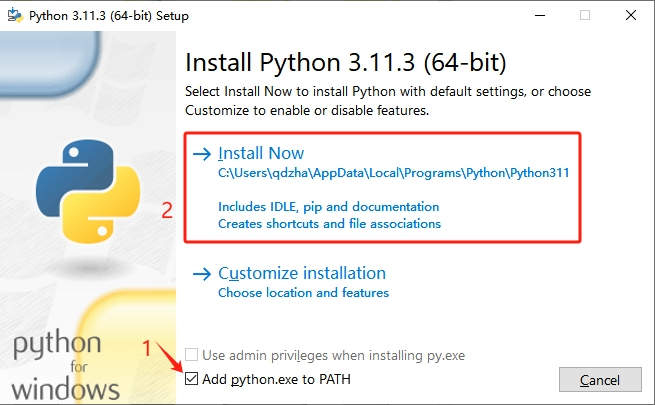
\includegraphics[width=1\linewidth]{Python与机器学习/基础Python语法/安装Python/fig/Python-IDLE安装.png}
    \caption{Python-IDLE安装}
    \label{fig:安装Python-Python-IDLE安装}
\end{figure}

\subsubsection{使用Anaconda安装Python}

相比于前面直接安装Python,安装Anaconda更有助于后续的学习。因此我们建议读者(尤其是面向科研的工作人员)安装Anaconda。

在安装Anaconda时,可以前往Anaconda的官网\footnote{https://www.anaconda.com/download},在网页中可能会需要提供邮箱,但提供与否并不影响实际下载。我们可以选择下方的“skip registration”进入下载页面。选择对应的操作系统版本点击下载即可。

\begin{attention}
    这里面的版本可能会与需要使用的版本不同,将在后面介绍如何在Anaconda中使用特定的Python版本(创建虚拟环境)。在这里不必担心所下载具体Python版本。
\end{attention}

下载完成后打开安装程序,如同正常的安装过程默认安装即可,在勾选选项时(如图\ref{fig:安装Python-Anaconda安装}所示)建议选择与图示相同的选项,点击“Install”安装即可。安装完成后可以在开始菜单找到“Anaconda”目录,打开其中的“Anaconda Prompt”,输入\code{python --version},若出现正常的版本号,则表明安装成功。

\begin{figure}
    \centering
    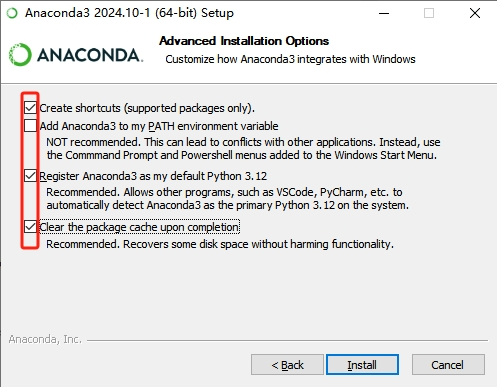
\includegraphics[width=1\linewidth]{Python与机器学习/基础Python语法/安装Python/fig/Anaconda安装.png}
    \caption{Anaconda安装}
    \label{fig:安装Python-Anaconda安装}
\end{figure}

\begin{extend}
    正如前面所说,在安装Anaconda时我们没有指定具体的Python版本,而在使用Anaconda时,可以通过创建虚拟环境指定代码运行时所使用的版本。具体创建方法为:

    \begin{enumerate}
        \item 在“Anaconda Prompt”中使用命令\code{conda create -n [环境名] python=[版本号]}创建对应的版本环境,例如,以3.11为例,使用\\\code{conda create -n py311 python=3.11},完成后输入“y”安装对应包即可下载对应版本的Python;
        \item 完成后输入\code{conda activate [环境名]}即可激活刚才所创建的环境。例如,以刚才所创建的环境为例,输入\code{conda activate py311}即可切换至环境中。切换后在命令行前面应当会有以括号开头的环境名表示当前环境;
        \item 在当前环境下输入\code{python --version}查看对应安装版本。
    \end{enumerate}
\end{extend}

\subsection{运行第一个Python程序}\label{subsec:安装Python-运行第一个Python程序}

下面,我们将测试自己所下载的Python是否可用,一个最简单也“约定俗成”的一段代码是“Hello World!”程序,即\emph{尝试输出“Hello World!”字符串}。针对上述两种安装方法,我们可以有不同的运行方式:

\subsubsection{使用命令行模式}

对于直接安装Python的用户而言,可以在开始菜单找到Python的IDLE,这是一个简单的集成开发环境。当你打开时,可以看到如图\ref{fig:安装Python-IDLE窗口}所示的IDLE窗口,前面的\code{>>>}表示等待输入命令。对于输出Hello World,可以执行下面的命令:

\code{print("Hello World!")}

输入后点击回车,在下方应当输出了“Hello World!”,从而表明Python安装正确。

\begin{figure}
    \centering
    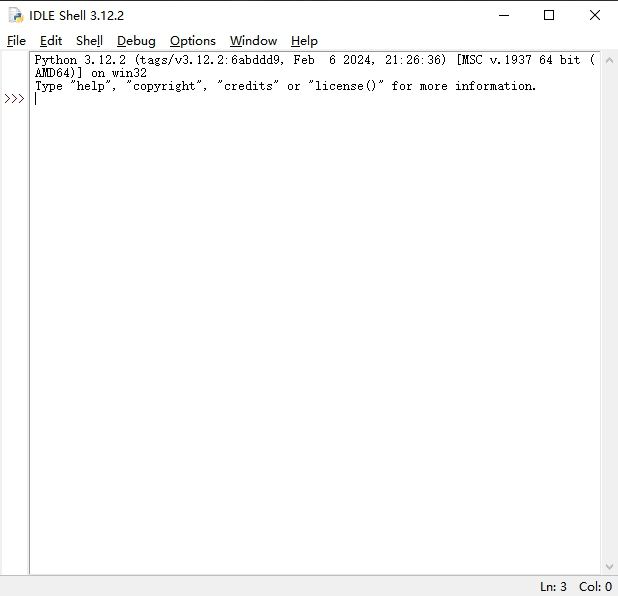
\includegraphics[width=1\linewidth]{Python与机器学习/基础Python语法/安装Python/fig/IDLE窗口.png}
    \caption{IDLE窗口}
    \label{fig:安装Python-IDLE窗口}
\end{figure}

\begin{attention}
    与其他编程语言类似,在编写Python程序时,请务必确保你的符号(引号内的文字可以除外)都是\emph{英文半角符号}。
\end{attention}

如果使用的Anaconda,则在打开Anaconda Prompt并激活环境后,输入\code{python}也可进入类似于上方IDLE的环境,可以执行正常的命令编写。与上面的步骤类似,可以执行\code{print("Hello World!")}查看输出结果

\begin{attention}
    在Anaconda Prompt当中,如果要退出Python则可以输入\code{exit()}或\code{quit()}退出至普通命令行模式。
\end{attention}

\subsubsection{使用文件模式}

上面的命令行只能适用于比较简单的命令测试,对于后面我们所学习的编程,大多数情况下是需要编写Python文件的。Python语言程序文件的后缀名是\code{*.py}。对于使用IDLE的用户,可以使用菜单栏的“File”-“New File”\footnote{或者使用快捷键Ctrl+N}创建一个文本文件。之后的编程则是在这个文本文件中进行。

以“Hello World!”为例,编写下面的文件并保存为\code{hello.py}文件

\begin{lstlisting}[language=python,numbers=left,caption={hello.py}]
print("Hello World!")
\end{lstlisting}

保存后点击上方的“Run”-“Run Module”(或者使用快捷键F5),则可以在前面的IDLE窗口中看到如下输出:

% \begin{lstlisting}
% =================== RESTART: C:/Users/qdzha/Desktop/hello.py ===================
% Hello World!
% \end{lstlisting}

\begin{lstlisting}
====== RESTART: C:/Users/qdzha/Desktop/hello.py ======
Hello World!
\end{lstlisting}

其中,第一行表示运行的程序路径与文件名,后面则是正常的程序执行过程(在这里输出“Hello World!”)

如果你使用的是Anaconda Prompt,则可以在外面使用文本编辑器(如记事本等)输入上面的程序并保存为\code{hello.py}(注意修改后缀名),然后再Anaconda Prompt的对应环境中输入命令:\code{python [程序路径名]}即可运行。

\begin{extend}
    虽然我们没有详细介绍关于Windows操作系统下的命令行操作,但在第一部分的\ref{subsec:通配符-使用通配符进行文件目录操作}一节中我们稍微提到了关于cmd的一些命令。与Linux类似,在使用Anaconda Prompt进行目录与文件操作时,在目录相关操作中(打开目录、切换上一级目录)与Linux系统的命令完全相同。

    因此,你可以在Anaconda Prompt当中使用\code{cd}命令打开至你所保存程序的目录。但是需要注意的是,由于Windows操作系统中硬盘分区的问题,当你希望切换至其他盘符时(例如,从C盘切换至D盘),则直接输入\code{d:}即可。在切换盘符后再切换回来时会保留你上一次的目录。

    在执行\code{python [程序路径名]}时,这个路径名可以是绝对路径(从盘符开始算起),也可以是相对路径名(从当前命令行所在目录开始算起)
\end{extend}

\subsubsection{*使用Anaconda Spyder编辑器}

这一部分是针对于Anaconda用户的,主要是为了方便文本编辑和程序运行测试。Spyder是一个使用Python语言的跨平台的科学运算集成开发环境,相比于其他编辑器,Spyder在调试代码时包含一个“工作空间”,方便对变量的值进行调试(类似于MATLAB)。

但在使用Spyder之前,我们需要做一点准备工作:首先,如果你使用的是自己创建的环境,在激活环境后\emph{需要安装spyder包},在Anaconda中,安装Spyder包的方法是在当前环境下输入\code{conda install spyder},搜索完必要包后输入“y”安装。

安装完成后在开始菜单打开Spyder(Anaconda目录下),找到对应的Spyder(一般括号后有对应的环境名)打开,即可进入界面如图\ref{fig:安装Python-Spyder界面}所示。类似于MATLAB界面,在右上角可以选择文件目录,点击上方菜单栏“文件”-“新建文件”可以创建Python程序。输入上面的Hello.py程序并保存即可创建文件。

\begin{figure}
    \centering
    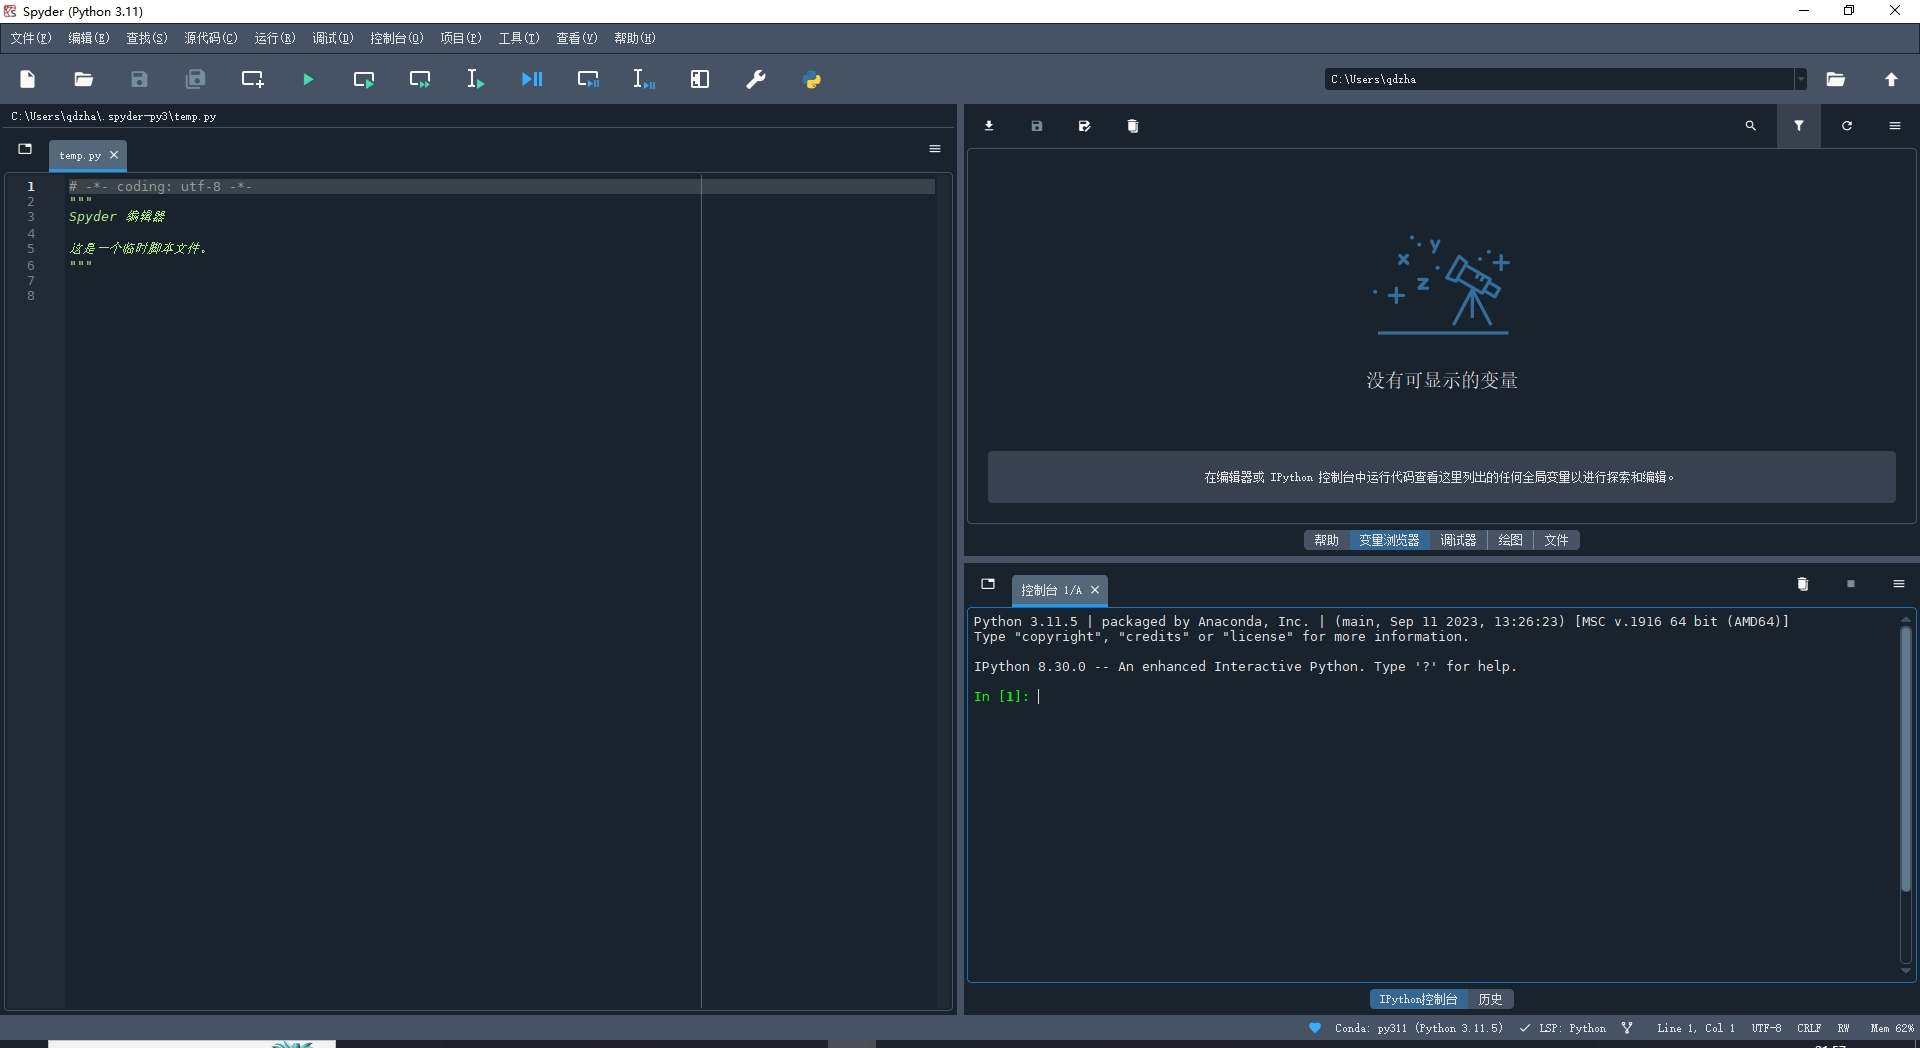
\includegraphics[width=1\linewidth]{Python与机器学习/基础Python语法/安装Python/fig/Spyder界面.png}
    \caption{Spyder界面}
    \label{fig:安装Python-Spyder界面}
\end{figure}

运行文件时,可以点击上方的“运行文件”图标,或使用快捷键F5,即可在右侧控制台看见对应的输出。

\begin{extend}
    除此之外,你也可以使用Anaconda Navigator工具来管理环境与使用Spyder。这个工具是使用窗口的方式进行操作,因此更加人性化。在开始菜单打开Anaconda Navigator后,如图\ref{fig:安装Python-Anaconda Navigator界面}所示,点击上方的下拉选项,选择需要切换的环境,找到Spyder启动即可(如果没有安装对应的包则会提醒“Install”安装。

    \begin{figure}
        \centering
        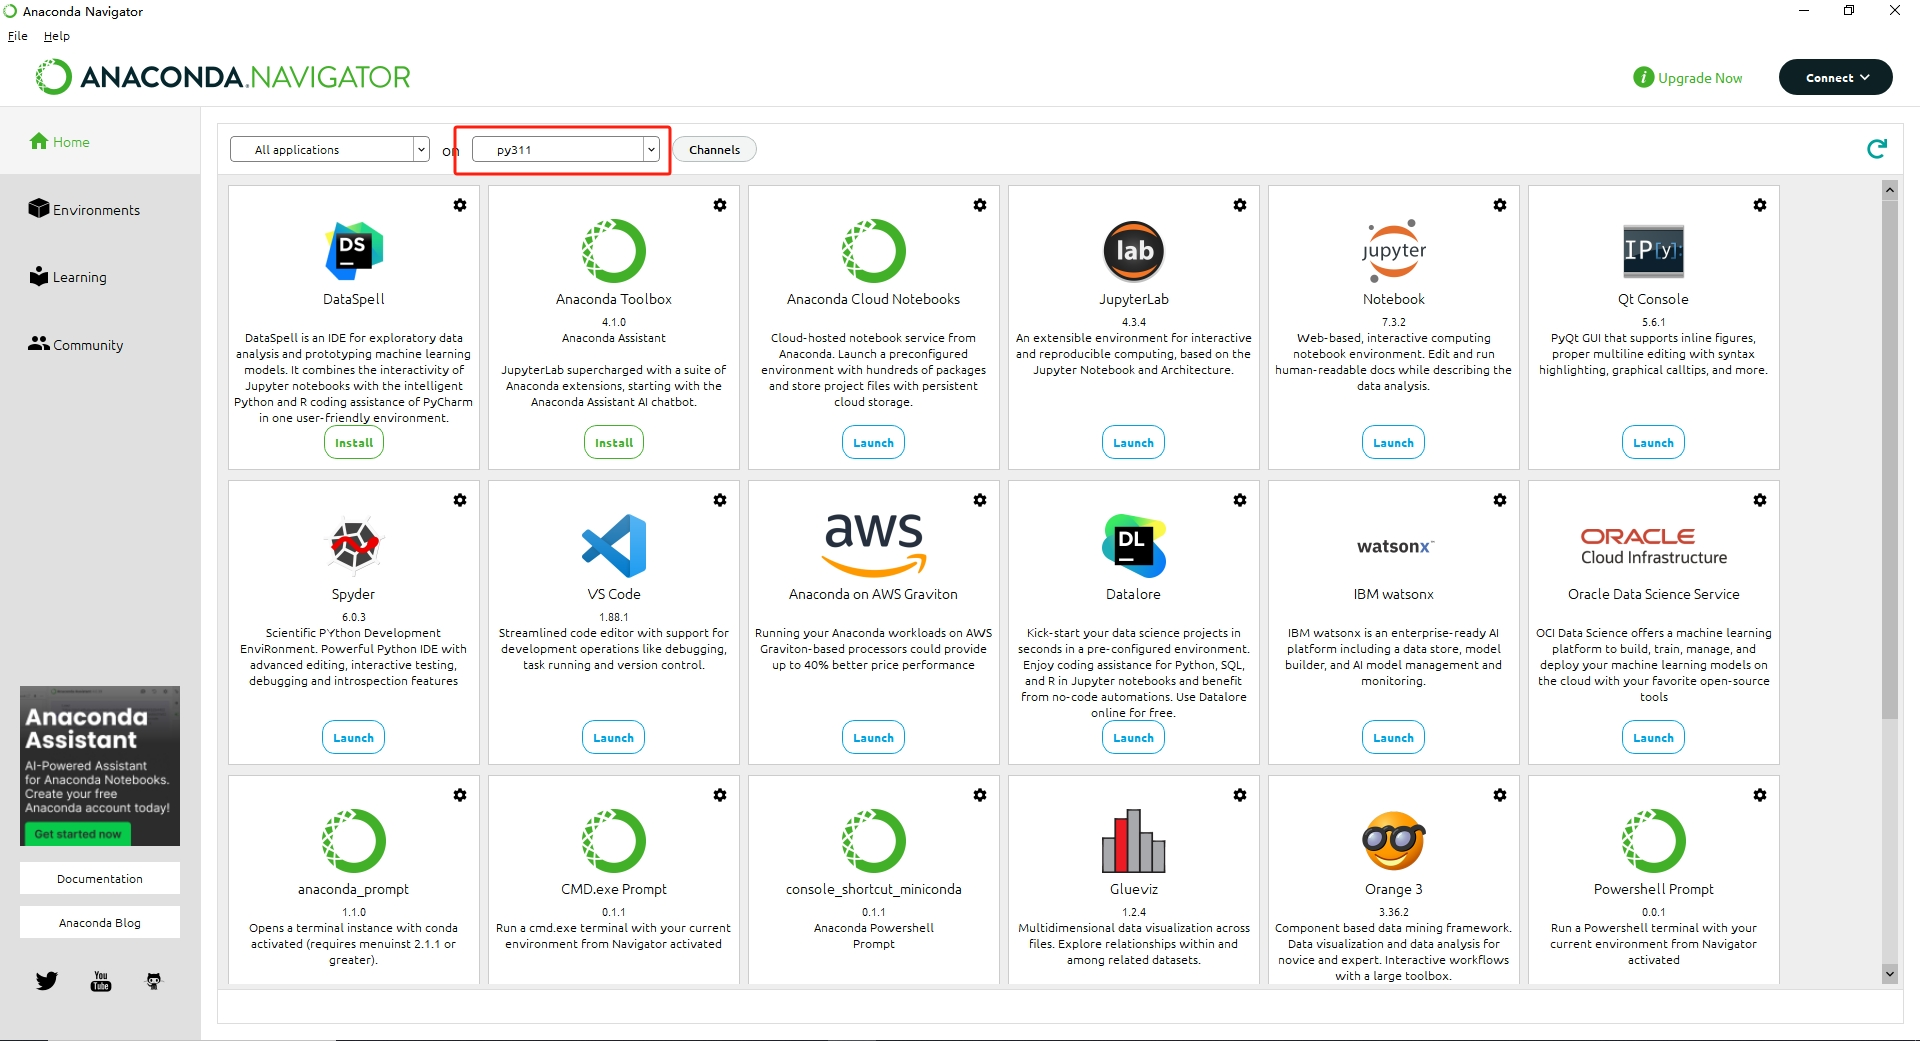
\includegraphics[width=1\linewidth]{Python与机器学习/基础Python语法/安装Python/fig/Anaconda Navigator界面.png}
        \caption{Anaconda Navigator界面}
        \label{fig:安装Python-Anaconda Navigator界面}
    \end{figure}

    在第二章以及后面的章节中可能会使用到另外的工具——Jupyter Notebook(或者Jupyter Lab),你也可以使用这种方式来安装并执行(相比于安装Jupyter内核,这种方式更加容易上手),在后面的章节我们将不会介绍如何在对应环境下启动Jupyter Notebook。
\end{extend}



\subsection{练习题}\label{subsec:安装Python-练习题}

\begin{itemize}
    \item [01] Python语言所使用的文件后缀名是什么?
    \item [02] 本节介绍了哪两种运行Python程序的方式?各有什么优劣?
    \item [10] 如果需要使用Anaconda创建一个名字叫“Exercise”的虚拟环境,Python版本为3.12,应当如何创建?
    \item [21] 在Anaconda中,可以使用\code{conda env list}查看所创建的虚拟环境及其对应的目录。尝试使用对应的目录,在cmd模式下使用对应的虚拟环境,并执行前面所编写的程序。
    [提示:不同的环境目录下都有一个\code{python.exe}文件,与cmd执行Python程序时的命令\code{python}是一样的]
    \item [P03] 仿照正文中的程序,编写一个Python程序,输出“Hello Python”。
    \item [P25] 在Python2和Python3当中,一个最大的区别是输出的方式不一样。对于Python3(前文所介绍的)是使用\code{print()}函数输出,输出内容作为函数的参数(在后面的章节中我们会详细介绍函数);而对Python2而言,使用的是\code{print}语句,即\code{print [字符串]}的方式。请使用Anaconda创建一个Python2.7的虚拟环境(尽管现在不建议),重写上面的“hello.py”程序,使其在Python2.7版本下可以正常输出“Hello World!”
    \item [16] 如果你下载使用的是Python IDLE,在下载时曾设置“Add Python.exe to PATH”。事实上这个PATH在Windows操作系统中可以通过右键单击“此电脑”-“属性”-“高级系统设置”-“环境变量”查看。请尝试查找对应的目录在哪里?如果删除掉这个环境变量会发生什么?
    \item [P18] 对于课题组内的服务器而言,有些服务器已经配置了Python或者Anaconda,请尝试在Linux服务器中编写正文中所提到的“Hello World!”程序。
    [提示:你可以通过\code{python --version}输出版本号的方式检查是否安装并可以正常调用Python。]
\end{itemize}

\subsection{错误处理}\label{subsec:安装Python-错误处理}

\subsubsection{SyntaxError: invalid character}

这种错误可能是由于你错误使用了符号字符,例如,当你在输入括号时使用中文括号,则会触发这个错误。因此,\emph{在编写程序时,除引号内,不要使用中文输入法}。